\clearpage
\appendix
\section{Additional figures and tables}
\label{app:figures}

\begin{table}[H]
  \centering
  \small
  \setlength{\tabcolsep}{2.6pt}
  \begin{tabular}{lrrrrcccc}
    \toprule
    & \multicolumn{4}{c}{Cost} & \multicolumn{2}{c}{\texttt{down\_proj}, layers 0 / 13 / 27} & \multicolumn{2}{c}{$R(z)$ math / non-math} \\
    \cmidrule(lr){2-5}\cmidrule(lr){6-7}\cmidrule(lr){8-9}
    Condition & params & min & GiB & state & $\rho_k$ & $100\,\eta$ & layer 13 & layer 27 \\
    \midrule
    Full FT, mid & & & & & .133 / .148 / .116 & 1.33 / 1.54 / 1.24 & .055 / .030 & .020 / .028 \\
    Full FT & 596M & 20.5 & 72.1 & 2.4\,GB & .133 / .148 / .115 & 1.37 / 1.60 / 1.29 & .056 / .031 & .020 / .028 \\
    + L2-SP & 596M & 21.0 & 74.4 & 2.4\,GB & .133 / .149 / .107 & 1.11 / 1.37 / 0.79 & .046 / .028 & .019 / .025 \\
    LoRA-4 & 2.5M & 17.8 & 64.5 & 10\,MB & .134 / .127 / .098 & 0.84 / 1.33 / 0.67 & .082 / .021 & .005 / .004 \\
    LoRA-16 & 10.1M & 17.8 & 64.6 & 40\,MB & .135 / .146 / .104 & 1.47 / 1.94 / 1.14 & .090 / .028 & .012 / .012 \\
    OPLoRA-16 & 10.1M & 19.4 & 64.9 & 40\,MB & $<10^{-6}$ & 1.46 / 1.96 / 0.92 & .100 / .030 & .011 / .011 \\
    \bottomrule
  \end{tabular}
  \caption{\textbf{Task 1 cost and local update geometry.} Trainable parameters, training minutes, peak allocated memory and saved state, measured at microbatch 16 $\times$ 2 (not the prescribed 2 $\times$ 16). L2-SP adds a 2.4\,GB copy of $\theta_0$ and 0.5\,min of penalty time. OPLoRA adds an 11.5\,s SVD, 323\,MB of bases and per-forward projections (most of its extra 1.6\,min). $\rho_k$: share of $\|\Delta W\|_F^2$ in the top-128 output directions of $W_0$ (random: 0.125); $\eta=\|\Delta W\|_F/\|W_0\|_F$; $R(z)=\|\Delta Wz\|_2/\|W_0z\|_2$, mean over 32 GSM8K and 32 HellaSwag probes. Sources: \file{resources.csv}, \file{diagnostics\_*.csv}.}
  \label{tab:task1diag}
\end{table}



\begin{figure}[H]
  \centering
  \begin{minipage}[b]{0.56\linewidth}
    \centering
    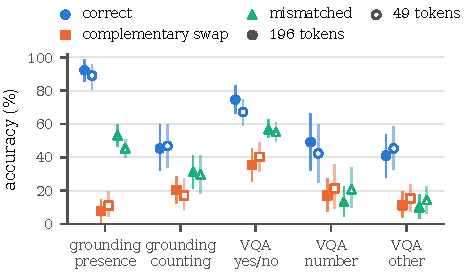
\includegraphics[width=\linewidth]{fig_task2_types.pdf}
  \end{minipage}\hfill
  \begin{minipage}[b]{0.42\linewidth}
    \small
    \setlength{\tabcolsep}{3pt}
    \begin{tabular}{lcc}
      \toprule
      Type & best constant & correct image \\
      \midrule
      presence & 50.0 (``yes'') & 92.2 \\
      counting & 28.1 (``1'') & 45.3 \\
      VQA yes/no & 50.0 (``no'') & 74.6 \\
      VQA number & 29.2 (``2'') & 49.2 \\
      VQA other & 8.3 (``red'') & 41.0 \\
      \bottomrule
    \end{tabular}
    \vspace{14pt}
  \end{minipage}
  \caption{\textbf{Accuracy by question type.} Left: accuracy (\%) under the three inputs that yield short answers, with 95\% pair-bootstrap intervals; filled markers 196 visual tokens, hollow the optional 49-token run. Right: best single answer for each type, as a question-only model could give, against correct-image accuracy. Sources: \file{eval\_final.json}, \file{t2\_constant\_baselines.csv}.}
  \label{fig:task2types}
\end{figure}



\begin{table}[H]
  \centering
  \footnotesize
  \setlength{\tabcolsep}{3pt}
  \begin{tabularx}{\linewidth}{>{\raggedright\arraybackslash}Xccccl}
    \toprule
    Question (type) & reference & correct & swap & unrelated & no image (image A) \\
    \midrule
    Does this image contain a toilet? (presence) & yes / no & yes / no & no / yes & no / no & ``No, the image does not\dots'' \\
    How many airplanes can you see? (counting) & 1 / 2 & 2 / 2 & 2 / 2 & 1 / 1 & ``The number \dots\ depends\dots'' \\
    Is this a kitchen? (VQA yes/no) & no / yes & no / yes & yes / no & no / no & ``No, this is not a kitchen.'' \\
    Umbrellas block what? (VQA other) & sun / rain & traffic / traffic & traffic / traffic & doors / board & ``\dots\ to block **rain**.'' \\
    \bottomrule
  \end{tabularx}
  \caption{\textbf{First complementary pair of each type} (answers for image A / image B). The VQA number pair, whose source question is malformed, is discussed in the text. Source: \file{eval\_final\_examples.jsonl}.}
  \label{tab:task2ex}
\end{table}



\begin{table}[H]
  \centering
  \small
  \setlength{\tabcolsep}{4pt}
  \begin{tabular}{llcccc}
    \toprule
    & & \multicolumn{3}{c}{accuracy (\%) at $N$} & $N=32$ minus \\
    \cmidrule(lr){3-5}
    Dataset & Rule & 4 & 8 & 32 & self-consistency (pp) \\
    \midrule
    \multirow{5}{*}{MATH}
      & self-consistency          & 69.2 & 71.8 & 73.8 & \\
      & highest mean log-prob     & 67.2 & 67.5 & 64.0 & $-9.8$ \ci{$-12.4$}{$-7.4$} \\
      & highest self-certainty    & 68.8 & 70.1 & 70.6 & $-3.2$ \ci{$-5.5$}{$-0.8$} \\
      & self-certainty + RWC      & 69.7 & 72.9 & 75.6 & $+1.8$ \ci{0.7}{2.9} \\
      & shortest rollout          & 65.2 & 64.6 & 62.4 & $-11.4$ \ci{$-14.1$}{$-9.0$} \\
    \midrule
    \multirow{8}{*}{MathVista}
      & self-consistency          & 58.0 & 60.5 & 63.1 & \\
      & highest mean log-prob     & 53.2 & 51.9 & 48.1 & $-15.0$ \ci{$-18.0$}{$-11.9$} \\
      & highest self-certainty    & 55.0 & 54.8 & 54.6 & $-8.5$ \ci{$-11.5$}{$-5.5$} \\
      & self-certainty + RWC      & 56.9 & 60.6 & 63.8 & $+0.7$ \ci{$-0.7$}{2.3} \\
      & highest vision $V$        & 54.5 & 54.3 & 53.6 & $-9.5$ \ci{$-12.6$}{$-6.4$} \\
      & vision + RWC              & 56.7 & 60.5 & 63.9 & $+0.8$ \ci{$-0.8$}{2.3} \\
      & highest VisConf           & 56.3 & 56.3 & 57.8 & $-5.4$ \ci{$-8.1$}{$-2.4$} \\
      & VisConf + RWC             & 57.9 & 61.1 & 64.5 & $+1.4$ \ci{$-0.1$}{2.8} \\
    \bottomrule
  \end{tabular}
  \caption{\textbf{Selection rules} on the 800 evaluation questions (first answer: 64.4 on MATH, 53.6 on MathVista). The last column is the paired difference from self-consistency at $N=32$ with its 95\% interval. Tokenwise VisConf $Z^{\mathrm{token}}$ (defined below) reaches 56.3 alone and 63.9 with RWC at $N=32$. Sources: \file{table\_methods\_*.csv}, \file{table\_bootstrap\_n32.csv}.}
  \label{tab:task3methods}
\end{table}



\begin{table}[H]
  \centering
  \small
  \setlength{\tabcolsep}{4pt}
  \begin{tabular}{lccccccc}
    \toprule
    Strategy (output allowance) & accuracy & answer found & truncated calls & input tok. & output tok. & seconds \\
    \midrule
    Single response (3,072)                & 0.58 & 0.96 & 2 / 50   & 108 & 682   & 31.7 \\
    Parallel, 3 $\times$ 1,024, vote       & 0.56 & 0.82 & 26 / 150 & 325 & 1,853 & 85.9 \\
    Refinement, 1,024 + 2,048              & 0.62 & 1.00 & 9 / 100  & 886 & 1,226 & 56.9 \\
    \bottomrule
  \end{tabular}
  \caption{\textbf{Live comparison on 50 MATH evaluation questions} (Qwen2.5-3B-Instruct, FP16, one NVIDIA L4, batch size 1; token counts and seconds are means per question). Refinement reuses the first parallel response as its initial answer and is charged for it. Paired differences: parallel minus single $-0.02$\ci{$-0.12$}{0.08}, refinement minus single $+0.04$\ci{$-0.08$}{0.16}, refinement minus parallel $+0.06$\ci{0.00}{0.14}. Source: \file{live\_summary.json}.}
  \label{tab:task3live}
\end{table}


